\section{662 --- Maximum Width of Binary Tree}
Given a binary tree, write a function to get the maximum width of the given tree. The width of a tree is the maximum width among all levels. The binary tree has the same structure as a full binary tree, but some nodes are null.

The width of one level is defined as the length between the end-nodes (the leftmost and right most non-null nodes in the level, where the null nodes between the end-nodes are also counted into the length calculation.

\paragraph{Example 1:}

\begin{flushleft}
\textbf{Input}:

\begin{figure}[H]
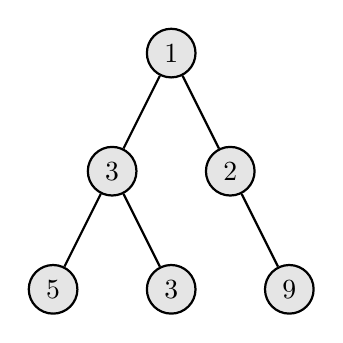
\begin{tikzpicture}
[every node/.style={draw, circle,
 minimum size=6mm, fill=gray!20!},
  node distance=8mm, 
  every join/.style={>=stealth,->},
 thick
]
\node{1}
child{node{3} child{node{5}} child{node{3}} }
child{node{2} child[missing] child{node{9}}};
\end{tikzpicture}
\end{figure} 

\textbf{Output}: 4

\textbf{Explanation}: The maximum width existing in the third level with the length 4  \lstinline[language=Java, basicstyle=\small\ttfamily, keywordstyle=\bfseries\color{green!40!black}]|(5,3,null,9)|.
\end{flushleft}

\paragraph{Example 2:}

\begin{flushleft}
\textbf{Input}: 

\begin{figure}[H]
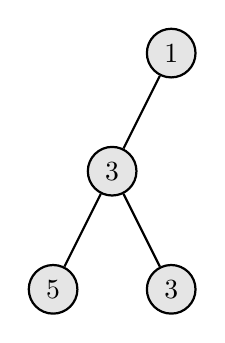
\begin{tikzpicture}
[every node/.style={draw, circle,
 minimum size=6mm, fill=gray!20!},
  node distance=8mm, 
  every join/.style={>=stealth,->},
 thick
]
\node{1}
child{node{3} child{node{5}} child{node{3}}}
child[missing];
\end{tikzpicture}
\end{figure}

\textbf{Output}: 2

\textbf{Explanation}: 

The maximum width existing in the third level with the length 2 (5,3).
\end{flushleft}

\paragraph{Example 3:}
\begin{flushleft}


\textbf{Input}: 

\begin{figure}[H]
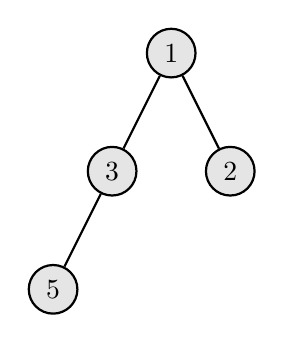
\begin{tikzpicture}
[every node/.style={draw, circle,
 minimum size=6mm, fill=gray!20!},
  node distance=8mm, 
  every join/.style={>=stealth,->},
 thick
]
\node{1}
child{node{3} child{node{5}} child[missing]}
child{node{2}};
\end{tikzpicture}
\end{figure}


\textbf{Output}: 2

\textbf{Explanation}: 

The maximum width existing in the second level with the length 2  \lstinline[language=Java, basicstyle=\small\ttfamily, keywordstyle=\bfseries\color{green!40!black}]|(3,2)|.
\end{flushleft}

\paragraph{Example 4:}

\begin{flushleft}


\textbf{Input}: 

\begin{figure}[H]
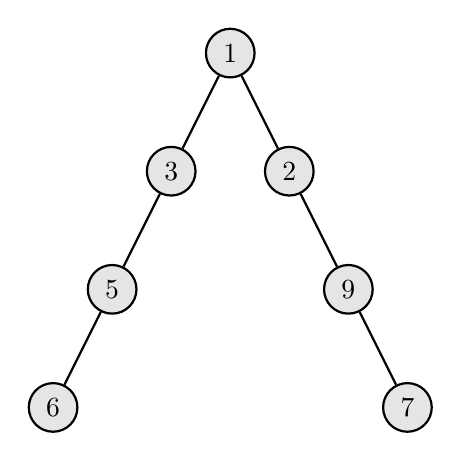
\begin{tikzpicture}
[every node/.style={draw, circle, minimum size=6mm, fill=gray!20!},
  node distance=8mm, 
  every join/.style={>=stealth,->},
 thick
]
\node{1}
child{node{3} child{node{5} child{node{6}} child[missing] } child[missing] }
child{node{2} child[missing] child{node{9} child[missing] child{node{7}} }  };
\end{tikzpicture}
\end{figure}
    
\textbf{Output}: 8

\textbf{Explanation}:

The maximum width existing in the fourth level with the length 8 

 \lstinline[language=Java, basicstyle=\small\ttfamily, keywordstyle=\bfseries\color{green!40!black}]|(6,null,null,null,null,null,null,7)|.
\end{flushleft}

\paragraph{Note:} 

\begin{itemize}
\item Answer will in the range of 32-bit signed integer.
\end{itemize}

\subsection{Breadth First Search}
We can assign each node a id. For example, the root node's id is zero and its left/right child's is 1 or 2 respectively. Specifically, if a node has a id $n$, the left and right child ids are $2n+1$ and $2n+2$ respectively.

On each level, get the first node's id $x$ and the last node's id $y$. The width is then $y-x+1$.

In C++ implementation, we may need  \lstinline[language=C++, basicstyle=\small\ttfamily, keywordstyle=\bfseries\color{green!40!black}]|unsigned long| as the type for id. It will fix the overflow for one test case.